\testCom
{%Номер задачи
	3.139
}
{%Условие
	условие
}
{%Дано
	дано
}
{%Найти
	найти
}
{%Решение
	%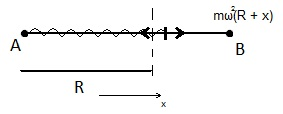
\includegraphics[height=30mm]{3_33.jpg}\\
	Очевидно, что контур теряет энергию из-за активного сопротивления (тепло) и эти потери описываются уравнением вида:\\
	$\der{Q}{t}{} = I^2 R$ - (закон Джоуля-Ленца), тогда искомая мощность $P = \der{Q}{t}{}, a \avr{P} = \frac{1}{T} \int\limits_0^T Q' \, dt$\\
	$\avr{P} = \frac{1}{T} \int\limits_0^T I^2 R \, dt = \frac{R}{T} \int\limits_0^T \dot q(t)\, dt$\\
	$q(t) = C U_m \sin \omega,$ где $\omega^2 = \frac{1}{LC}$, тогда\\
	$\der{q}{t}{} =U_m \omega C \cos \omega t \quad T = \frac{2 \pi}{\omega}$\\
	$\avr{P} = R \frac{2 \pi}{\omega} u^2 \omega^2 C^2 \int\limits_0^{\frac{2 \pi}{\omega}} \cos^2 \omega t \, dt = \frac{R U_m^2 C}{L} \frac{\omega}{2 \pi} \int\limits_0^{\frac{2 \pi}{\omega}} \frac{1 + \cos \omega t}{2} \, dt = \frac{C U_m^2 R}{2L}$\\	
}

